\documentclass[14pt]{article}

\usepackage[utf8x]{inputenc}
\usepackage[russian]{babel}
\usepackage{graphicx}
\graphicspath{{images/}}
\DeclareGraphicsExtensions{.pdf,.png,.jpg}

\usepackage{amsmath}
\usepackage{pgfplots}

\usepackage{geometry} % Меняем поля страницы
\geometry{left=2cm}% левое поле
\geometry{right=1.5cm}% правое поле
\geometry{top=2cm}% верхнее поле
\geometry{bottom=2cm}% нижнее поле

\renewcommand{\theenumi}{\arabic{enumi}}
\renewcommand{\labelenumi}{\arabic{enumi}}
\renewcommand{\theenumii}{.\arabic{enumii}}
\renewcommand{\labelenumii}{\arabic{enumi}.\arabic{enumii}.}
\renewcommand{\theenumiii}{.\arabic{enumiii}}
\renewcommand{\labelenumiii}{\arabic{enumi}.\arabic{enumii}.\arabic{enumiii}.}

\begin{document}
\begin{titlepage}
	\begin{center}
		\fontsize{18pt}{20pt}\selectfont
		\textbf{Работа 3.5.1.}	
	
		\vspace{5cm}
		\fontsize{24pt}{25pt}\selectfont
		Изучение плазмы газового разряда в неоне
	\end{center}
	\begin{flushright}
		\fontsize{18pt}{20pt}\selectfont
		\vspace{14cm}
		\hspace{-3cm}
		\textit{Корнеев Е.С.}
	\end{flushright}		
\end{titlepage}

\begin{center}
	\fontsize{16pt}{18pt}\selectfont	
	Изучение плазмы газового разряда в неоне
\end{center}


\fontsize{14pt}{16pt}\selectfont
\vspace{1cm}
\textbf{Цель работы:} изучение вольт-амперной характеристики тлеющего разряда; изучение свойств плазмы методом зондовых характеристик.

\vspace{0.5cm}
\textbf{Оборудование:} стеклянная газоразрядная трубка, наполненная изотопом неона, высоковольтный источник питания, источник питания постоянного тока, делитель напряжения, резистор, потенциометр, амперметры, вольтметры, переключатели. 

\vspace{1cm}
\textbf{Экспериментальная установка.} Схема установки для исследования плазмы газового разряда в неоне представлена на рисунке 1. Стеклянная трубка имеет холодный (ненакаливаемый) полый катод, три анода и геттерный узел - специальный баллон, на внутреннюю поверхность которого напылена газопоглощающая пленка (геттер).Трубка наполнена изотопом неона $^{22}$Ne при давлении 2 мм.рт.ст. Катод и один из анодов (I или II) с помощью переключателя П$_1$ подключается через балластный резистор 
$R_\text{б}~(\approx 450 \text{кОм})$ к регулируемому высоковольтному источнику питания (ВИП) с выходным напряжением до 3кВ. 

\begin{figure}[h!]
	\center{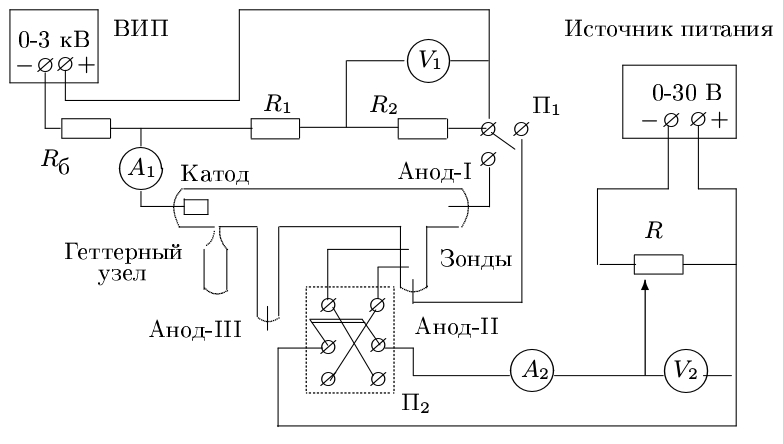
\includegraphics[width = 15cm]{1}}
	\caption{Схема установки}
	\label{fig:image}
\end{figure}

При подключении к ВИП анода-I между ним и катодом возникает газовый разряд. Ток разряда измеряется миллиамперметром $A_1$, а падение напряжения на разрядной трубке - цифровым вольтметром $V_1$ (В7-38), подключенным к трубке через высокоомный (25 МОм) делитель напряжения с коэффициентом $(R_1 + R_2)/R_2 = 10$.

При подключении к ВИП анода-II разряд возникает в пространстве между катодом и анодом-II, где находится двойной зонд, используемый для диагностики плазмы положительного столба. Зонды изготовлены из молибденовой проволоки диаметром $d = 0.2$ мми имеют длину $l = 5.2$ мм. Они подключены к источнику питания (0-30 В) через потенциометр $R$. Переключатель П$_2$ позволяет изменять полярность напряжения на зондах. Величина напряжения на зондах изменяется с помощью дискретного переключателя "$V$" выходного напряжения источника питания и потенциометра $R$, а измеряется вольтметром $V_2$. Для измерения зондового тока используется микроамперметр $A_2$. 

Анод-III в нашей работе не используется. 





















\end{document}